\cleardoublepage
\chapter{The rise of \ebook{}s} \label{ch:intro}

In the past five years, the surge in popularity of tablets and dedicated \ebook{} readers has vastly increased the sale and distribution of \ebook{}s.

In August 2012, it was widely reported in the media that Amazon's Kindle Store sales were outstripping print book sales by 114 to 100. This figure did not include free \ebook{}s `sold' through the Kindle Store, which would skew the figures significantly further.

Project Gutenberg, a digital online library that (at the time of writing) hosts over 43,000 freely downloadable \ebook{}s, regularly exceeds 150,000 downloads \emph{per day}.\footnote{See \url{http://www.gutenberg.org/browse/scores/pretty-pictures} for up-to-date statistics.}

\section{Devices}

In\marginpar{Amazon distributes software that allows Kindle format books to be read on Android and iOS tablets and smartphones, and on Windows and OS X, in addition to its own range of Kindle hardware} addition to dedicated \ebook{} readers, such as the Amazon Kindle and the Kobo eReader, many other devices  can be equipped to read \ebook{} files, such as tablets, mobile phones, laptops, and desktop PCs. Indeed, virtually every modern device with network connectivity and a screen can be equipped to read \ebook{}s.

The screen technologies used in these devices has vastly improved in the past decade or so, from the introduction of e-paper screens that provide a reading experience very similar to that of real paper, to the enormous advances in \textsc{lcd} and \textsc{oled} screens, which now often have pixel densities high enough that it is difficult to resolve individual pixels with the naked eye\ed Figure~\ref{fig:screens} shows some examples of document display technologies.

As a consequence of this, \ebook{} files must be flexible enough to allow their content to be be displayed and read on a vast range of devices with differing screen screen sizes and types.

\begin{figure}
    \captionsetup[subfigure]{justification=raggedright}
    \begin{centering}

        \subfloat[][A commercially printed book]{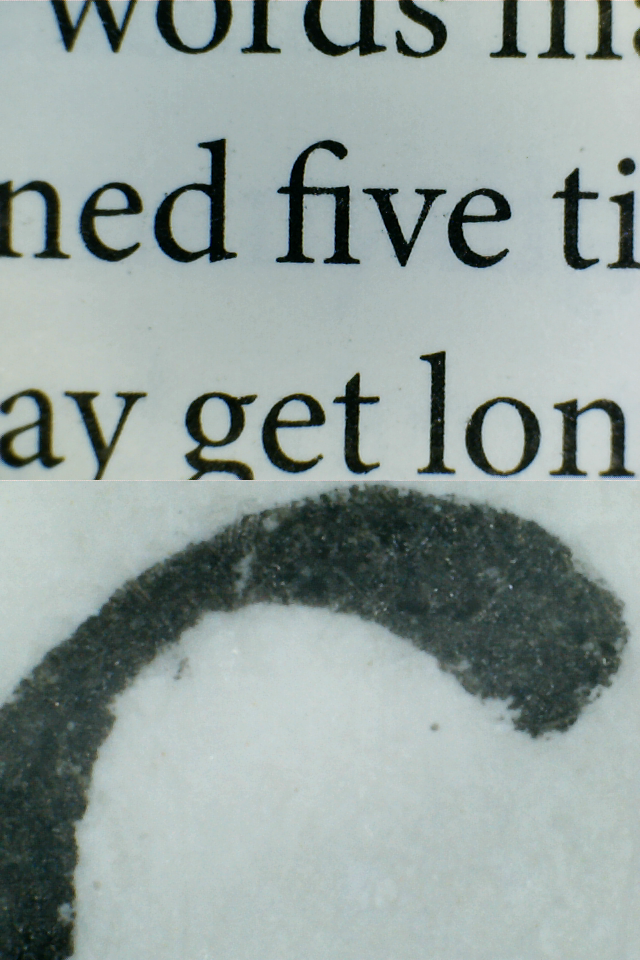
\includegraphics[width=0.3\textwidth]{gfx/sc-book}} \hspace{1mm} 
        \subfloat[][A laser-printed webpage]{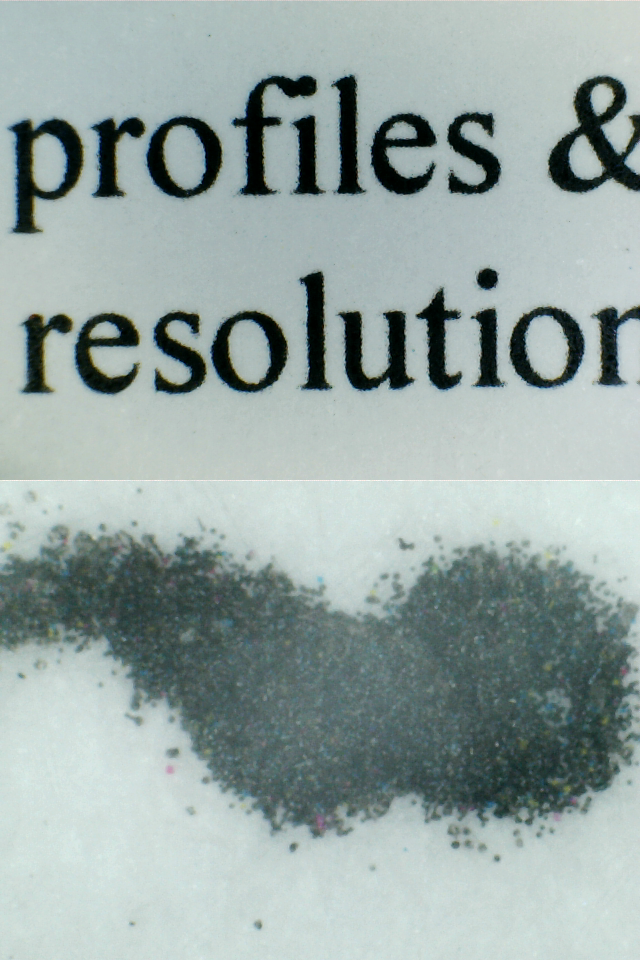
\includegraphics[width=0.3\textwidth]{gfx/sc-laser}} \hspace{1mm} 
        \subfloat[][A dot-matrix \textsc{lcd} screen]{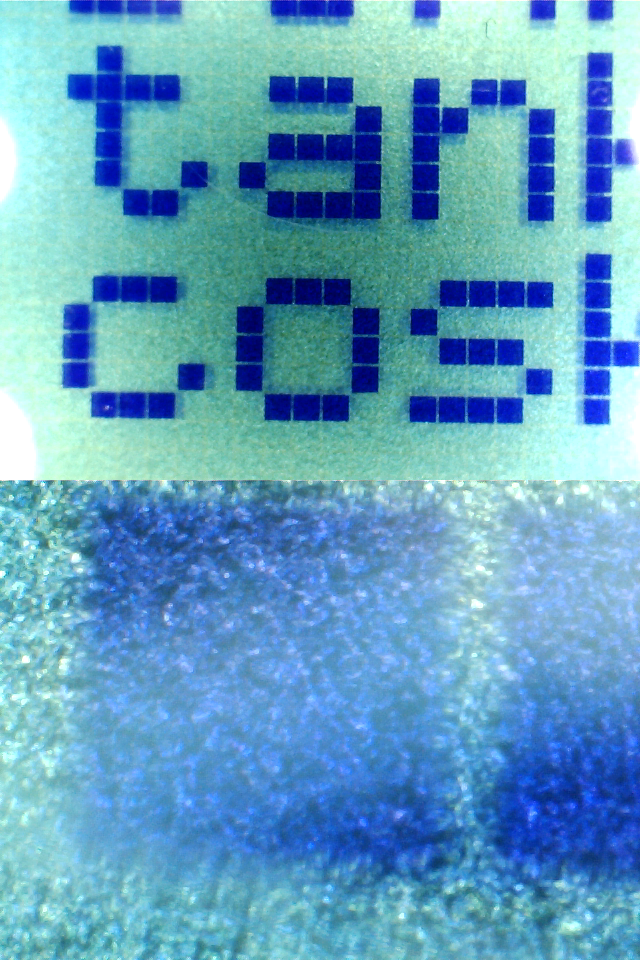
\includegraphics[width=0.3\textwidth]{gfx/sc-lcd}\label{fig:calculator}} 

        \subfloat[][A \textsc{tft} \textsc{lcd} monitor]{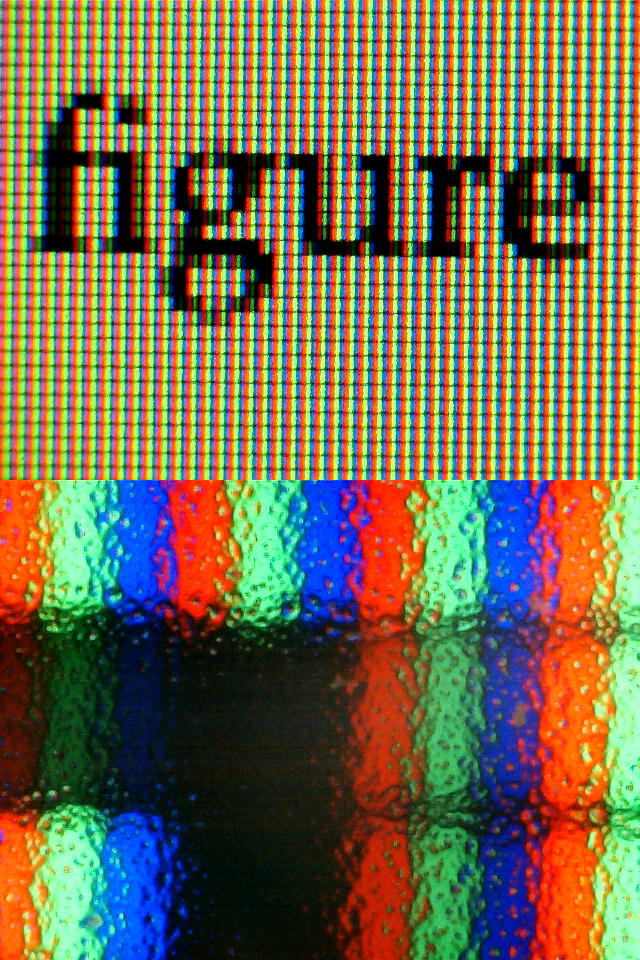
\includegraphics[width=0.3\textwidth]{gfx/sc-tft1}} \hspace{1mm} 
        \subfloat[][Another \textsc{tft} \textsc{lcd} monitor]{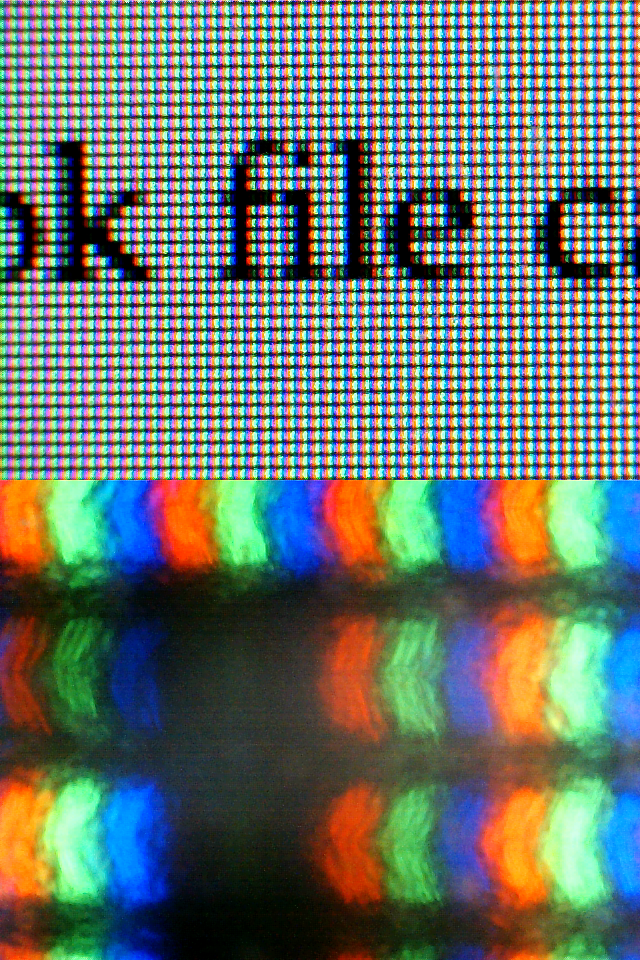
\includegraphics[width=0.3\textwidth]{gfx/sc-tft2}} \hspace{1mm} 
        \subfloat[][A \textsc{tft} \textsc{lcd} on a Kindle Fire HD]{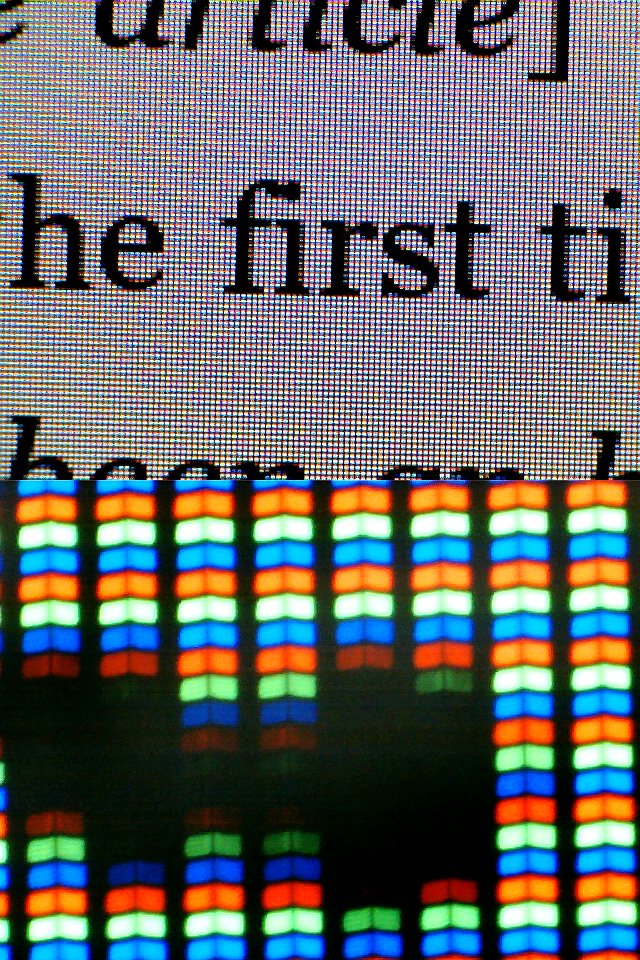
\includegraphics[width=0.3\textwidth]{gfx/sc-fire}} 

        \subfloat[][A Super \textsc{amoled} display on a Galaxy Nexus smartphone]{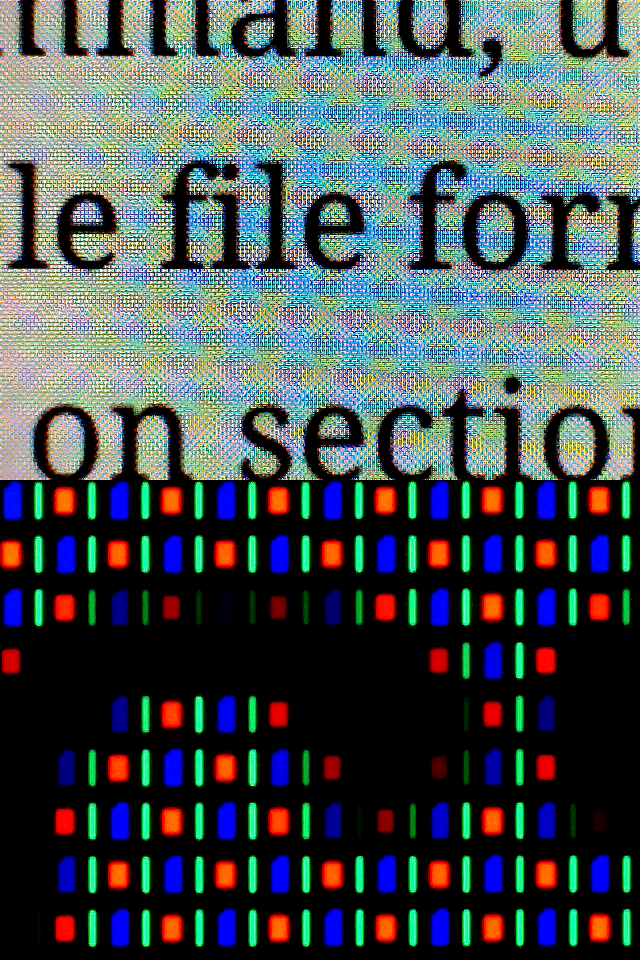
\includegraphics[width=0.3\textwidth]{gfx/sc-gnex}} \hspace{1mm} 
        \subfloat[][An e-paper screen on a Kobo eReader]{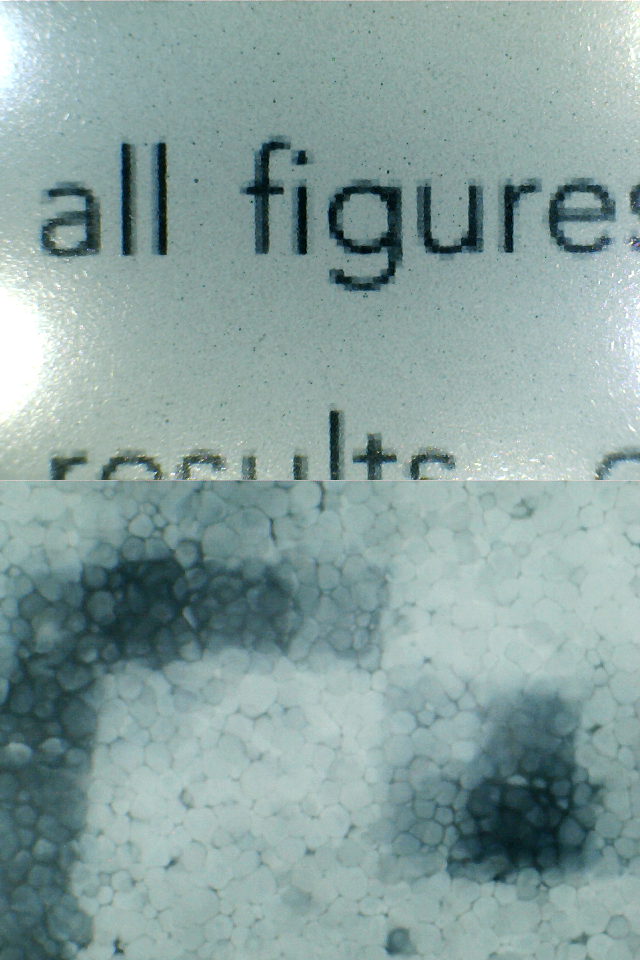
\includegraphics[width=0.3\textwidth]{gfx/sc-kobo}} \hspace{1mm} 
        \subfloat[][An e-paper screen on a Kindle Touch]{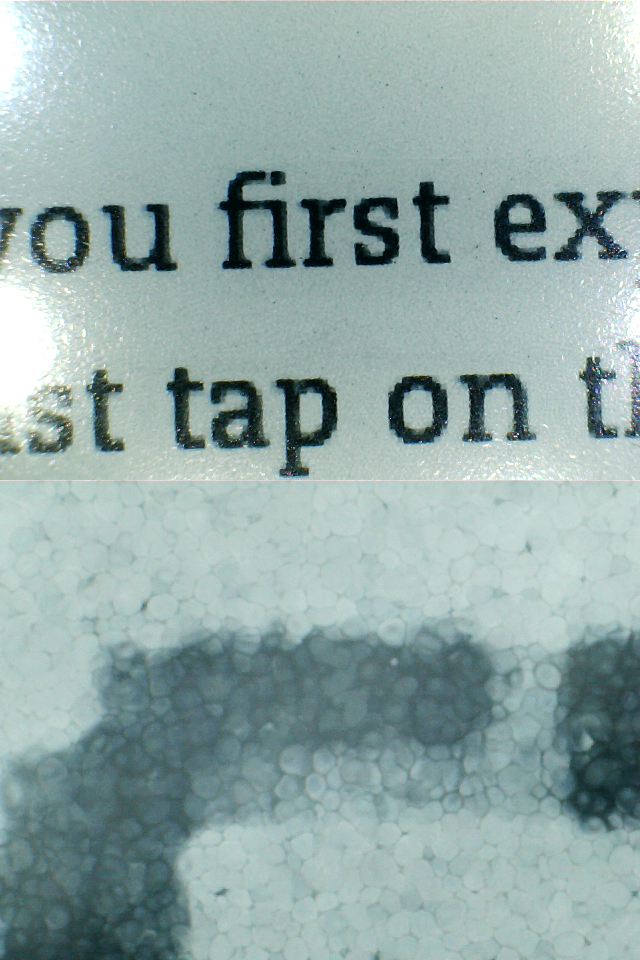
\includegraphics[width=0.3\textwidth]{gfx/sc-kindle}} 

    \end{centering}

    \caption[Examples of document display technologies]{Examples of some document display technologies, magnified about 25 times (top halves of images) and 350 times (bottom halves). Note that the resolution of the screen in (g) is close to that of the microscope used to capture the image, hence the aliasing effect.}
    \label{fig:screens}
\end{figure}




\section{Paradigms of Document Representation}
Computer representations of documents can be classified into two distinct paradigms:
\begin{itemize}
 \item Documents may be stored in \emph{fixed formats}, such as \pdf{} and PostScript, which are designed to be the direct analogue of printed pages
 \item Documents may be stored in \emph{flowable formats} such as \html{} and \epub{}, which have no fixed presentation associated with them, and whose layout must be computed each time the document is displayed
\end{itemize}
Currently there is no middle ground\ed a document may either be fully rendered to a fixed layout, or completely unrendered, to be laid out at the mercy of a display device's decisions.

\subsection{Fixed Formats}
\label{sec:fixedformats}
The only fixed document format commonly used for \ebook{}s (or indeed commonly used at all) is \pdf{}, which was originally designed as a way of faithfully reproducing documents both on screen and in print. For this reason, it is almost entirely pre\-s\-en\-ta\-tion-oriented and will not necessarily include any metadata pertaining to the semantic structure of a given document.

The archetypal \pdf{} file consists solely of drawing operators which describe the document pages. There is no compulsion for these drawing operators to render the page in an order that might be considered sensible by a human reader. For example, if a \pdf{} generator program decided to render every character on a page in alphabetical order, or radially outwards from the centre, the resulting file would still be semantically valid, and the result should be imperceptible to the end user.

This lack of imposed semantic structure makes it difficult to infer the best way to `unpick' \pdf{} files to allow their content to be reflowed into a new layout. For example, it is not easy to decide programatically whether the line break between adjacent lines of text is explicitly intended to be there, or whether the lines should logically flow together.

This is not to say that \pdf{} files \emph{cannot} represent the semantic structure of their content\ed indeed as early as 1999, \pdf{}~1.3 introduced \emph{logical structure} facilities,~\cite{Adobe2001} adding an optional \emph{structure tree} to the \pdf{} specification, and \emph{tagged \pdf{}}, introduced in \pdf{}~1.4 in 2001, provides various extensions to this. \pdf{} documents which actually make good use of these facilities are few and far between, even a decade after their introduction.

%Unfortunately, even when these facilities to include structural semantics are actually used, it is still not particularly useful in reflowing the content of documents. It is true that it helps to correctly identify the logical order of page components, but 

%If a document is stored at a higher, more abstract level than \pdf{}, the text can be rendered at any desired size, at the cost of the retention of high-quality typesetting afforded by \pdf{}.

\subsection{Flowable Formats}
\label{sec:flowableformats}
\marginpar{Amazon's proprietary Kindle format is derived from Mobipocket; \pdf{} and \epub{} are open standards}
The two most common flowable \ebook{} formats are \epub{} and Mobipocket, both of which are largely based on \html{}. \html{} was chosen not only because of its inherent support for reflow, but also because it allows document content to be semantically marked up into paragraphs, varying levels of headers, and so on. At the time, this was an enormous improvement over \ebook{}s stored as plain text, which consequently had no formatting \emph{or} semantic structure, 

Whilst the use of these \html{}-like formats allows the semantic structure of documents to be very well defined, in general their presentation can only be specified in a very loose manner. On an \ebook{} reader (or in \ebook{} reading software) the user is often presented with a choice of typefaces and point sizes, which gives the reader software scope to render the document in any number of arbitrary ways.

Since a document stored in a flowable format has no concrete presentation associated with it, each time the document is displayed, its layout must be recomputed. For an \ebook{} reader to maximise its battery life, this computation must be as simple as possible, \ie{} the algorithm used must not be too complex, since the more \textsc{cpu} cycles spent executing it, the less time the \textsc{cpu} can spend idle, and thus the greater the drain on the device's battery. Furthermore, the longer that is spent formatting the output, the longer the delay between page turns on the device, and with the speed of \textsc{cpu}s used in these devices ($<$ 500 \textsc{MHz}) it does not take too large an increase in computation for the page-turn time to become noticeable.



\section{Limitations of Current Formats}

The design paradigm of \pdf{}, conceived in the early 1990s,~\cite{Warnock1991} was to form a perfect analogue of the printed page, which would be exactly reproducible regardless of the system on which the file was rendered. For this reason, it is possible to embed fonts within \pdf{} files, to ensure faithful reproduction on any system, regardless of which fonts are actually installed. In general, a well typeset \pdf{} file looks good wherever it is displayed, but, stemming from the `digital sheet of paper' paradigm, page sizes in a \pdf{} document are necessarily fixed at creation-time. An overwhelming majority of \pdf{} documents are rendered for  US letter or A4 size paper. This is fine if the document is to be printed and read. On a reasonably large screen, the document remains perfectly readable, and a 10'' netbook or tablet screen may provide acceptable reading. Anything much smaller (notably mobile phones, and \ebook{} readers) requires a combination of zooming and panning  in order to read the document.

Documents may, of course, be rendered to a smaller page size, however the problem still remains\ed it is unlikely that any one page size will be suited to \emph{all} reading platforms. Most \ebook{} readers, using their native (i.e.\ non-\pdf{}) formats, allow text to be resized according to user preference. Indeed, it seems unnecessarily restrictive to force one size of type upon the user. Of course, paper books suffer from this affliction; digital books need not. Selling \ebook{}s separately in standard and large-print versions seems perverse when, for virtually no difference in cost to the publisher/distributor, both can be included in one file.

Applications have been written that attempt to reflow the content of PDF documents, but as noted in Section~\ref{sec:fixedformats}, this is often extremely difficult to accomplish satisfactorily. Even when the logical order of page components is correctly identified, the benefit of any precomputed high-quality typesetting is lost, since the text must be re-typeset.



\epub{} and Mobipocket, both based on \html{}, provide a higher abstraction of documents. This allows a font size to be chosen at view-time, and the text to be rendered accordingly, to closely fit the screen. Line breaks and page breaks can then be calculated and inserted as necessary, in order to wrap the text to fit the screen, and to paginate the content. The rendering engines of \ebook{} readers use simplistic reflow algorithms\ed but necessarily so.

The battery life of portable devices is lamentably low\ed battery capacity has not improved at anywhere near the same rate as other facets of mobile computing. Manufacturers of \ebook{} readers may claim their products have batteries which can last for weeks, but this is principally due to the many shortcuts used when laying out flowable content. As noted in Section~\ref{sec:flowableformats}, were these devices to use more complex layout algorithms, which can produce far higher quality typeset output, it would soon emerge that any savings made by using a low-power e-paper screen would quickly disappear. In addition to increasing battery usage, the higher computational complexity of these algorithms may cause page turns to take longer, as each subsequent page is only rendered when a page turn is requested. This time delay could be fixed reasonably easily by buffering between page turns, but this would not solve the battery drain problem.


\epub{} allows fonts to be embedded, but Mobipocket does not. Mobipocket files (and by extension, Kindle files) are therefore restricted to be rendered in a typeface local to (and often chosen by) the reader software. The Kindle, as an example, provides the user with a choice of `regular', `condensed', or `sans-serif' for the main body text of its documents. There are bold and italic variants of these, which are applied according to formatting instructions within the documents themselves. Additionally, there is a typewriter-style font which document authors may choose to use in the same manner. The Mobipocket specification supports a very limited subset of \html{} and \css{}, which makes it virtually impossible to achieve complex layouts such as those involving arbitrary indentation or font size changes. Figures \ref{fig:alices1} and~\ref{fig:alices2} demonstrate the well known `Mouse's Tale' from Lewis Carroll's \emph{Alice in Wonderland}, and the limitations of various formats.


\begin{figure}[tb]
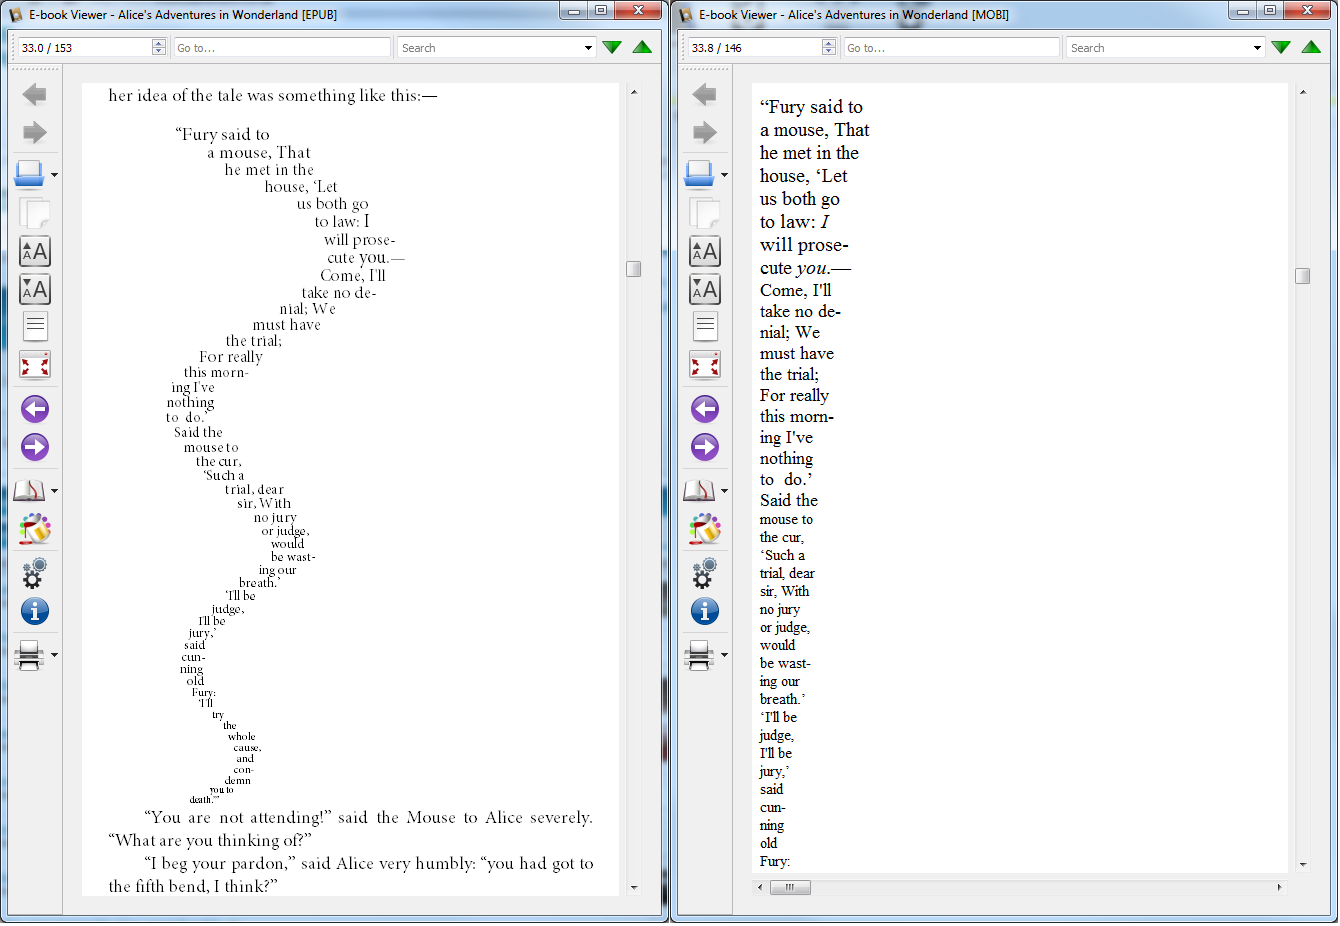
\includegraphics[width=\textwidth]{gfx/alices1}
\caption[Document displayed in Calibre]{On the left is an \epub{} version of Alice in Wonderland, displayed in Calibre (an open source desktop \ebook{} viewer). On the right is the same file, converted to Mobipocket, also displayed in Calibre. Note that in addition to the indentation being lost, the (embedded) font from the \epub{} is no longer present in the Mobipocket file.}
\label{fig:alices1}
\end{figure}

%\marginpar{Mobipocket\ed can't embed fonts... very limited choice of html to use. Reliant on
%rendering engine of device.
%\epub{}\ed can embed fonts, can style with \css{} pretty much arbitrarily, but still needs to be
%retypeset on each viewing and thus relies on the crappy built in rendering engine of the device.}

\epub{} is a little more flexible, since it supports a more comprehensive range of \xhtml{} and \css{}, and allows for arbitrarily complex styling. \epub{} files are still entirely reliant on the rendering engine of the display device correctly displaying their content, as they have no concrete layout associated with them.

\begin{figure}[tb]
\begin{center}
\vspace{-.3in}
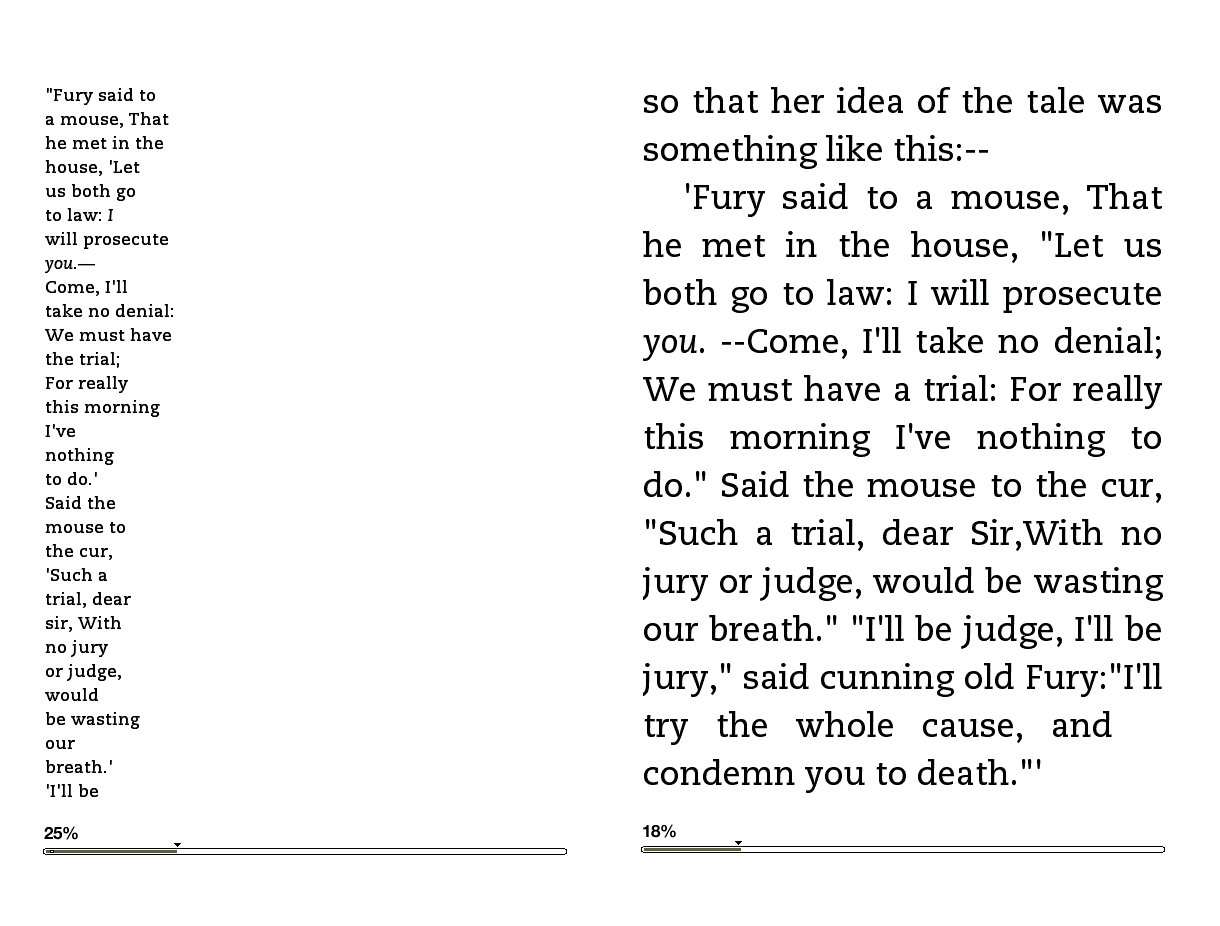
\includegraphics[width=\textwidth]{gfx/alices2}
\end{center}
\vspace{-.3in}
\caption[The same document displayed on the Kindle]{On the left is the Mobipocket version of Alice in Wonderland (from Figure~\ref{fig:alices1}) displayed on the Kindle. Note that the sizing instructions appear to have been ignored. On the right is the free version of Alice in Wonderland from the Kindle store, displayed on the Kindle. Note that no attempt has been made to render the poem in a `tail' shape.}
\label{fig:alices2}
\end{figure}

\section{``Good'' typesetting}
\label{sec:goodtypesetting}

\begin{figure}
    \centering
    \fbox{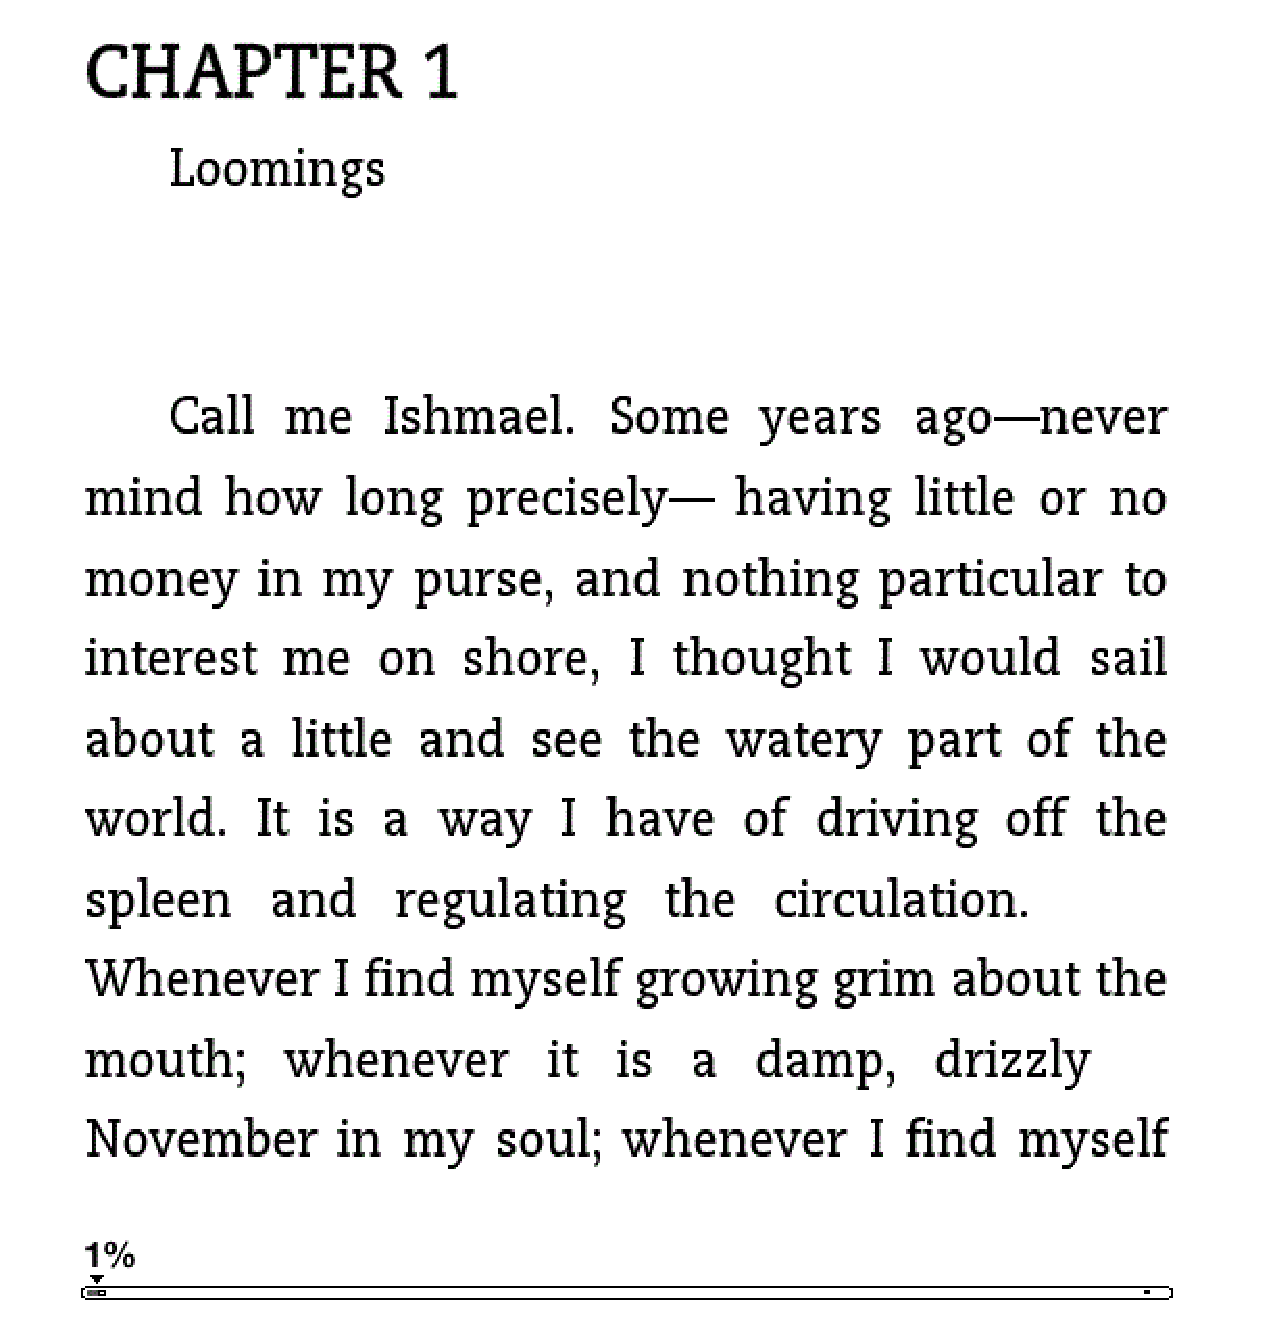
\includegraphics[width=\textwidth
]{gfx/screen_shot-42583}}
    \caption[Poor typography on the Kindle]{The Kindle Keyboard appears to primarily use justified text, falling back to ragged-right when inter-word spacing would become too large.}
    \label{fig:crapkindle}
\end{figure}

\subsection{Hyphenation and Line-Breaking}
\Ebook{} readers typically use a `greedy' algorithm to lay out their text\ed that is, they place as many words as will fit onto the current line without exceeding it, then start a new line and continue. Although this algorithm is optimal in that it will always fit text onto the fewest possible lines, it often causes consecutive lines to have wildly varying lengths, accentuating either the `ragged-right' effect of the text, or, in the case of justified text, the inter-word spacing. In general, \ebook{} readers will only hyphenate in extreme cases\ed indeed the Kindle Keyboard seems not to do so at all, to the detriment of its typography (see Figure~\ref{fig:crapkindle}).

Donald E. Knuth and Michael F. Plass~\cite{Knuth1981} developed a more advanced line-breaking algorithm (now used by \TeX{}) which attempts to minimise large discrepancies between consecutive lines by considering each paragraph as a whole. \TeX{} also uses the hyphenation algorithm designed by Franklin Liang~\cite{Liang1983} (another of Knuth's grad students) which has been ported to many other applications.

Knuth and Plass's line breaking algorithm, in conjunction with Liang's hyphenation algorithm, breaks paragraphs into lines of text to fit a page, resulting in what can be considered an aesthetically optimal configuration. \TeX 's default behaviour is then to alter the spacing between words in order to justify the line to fit the measure of the page.

\begin{figure}
 \fbox{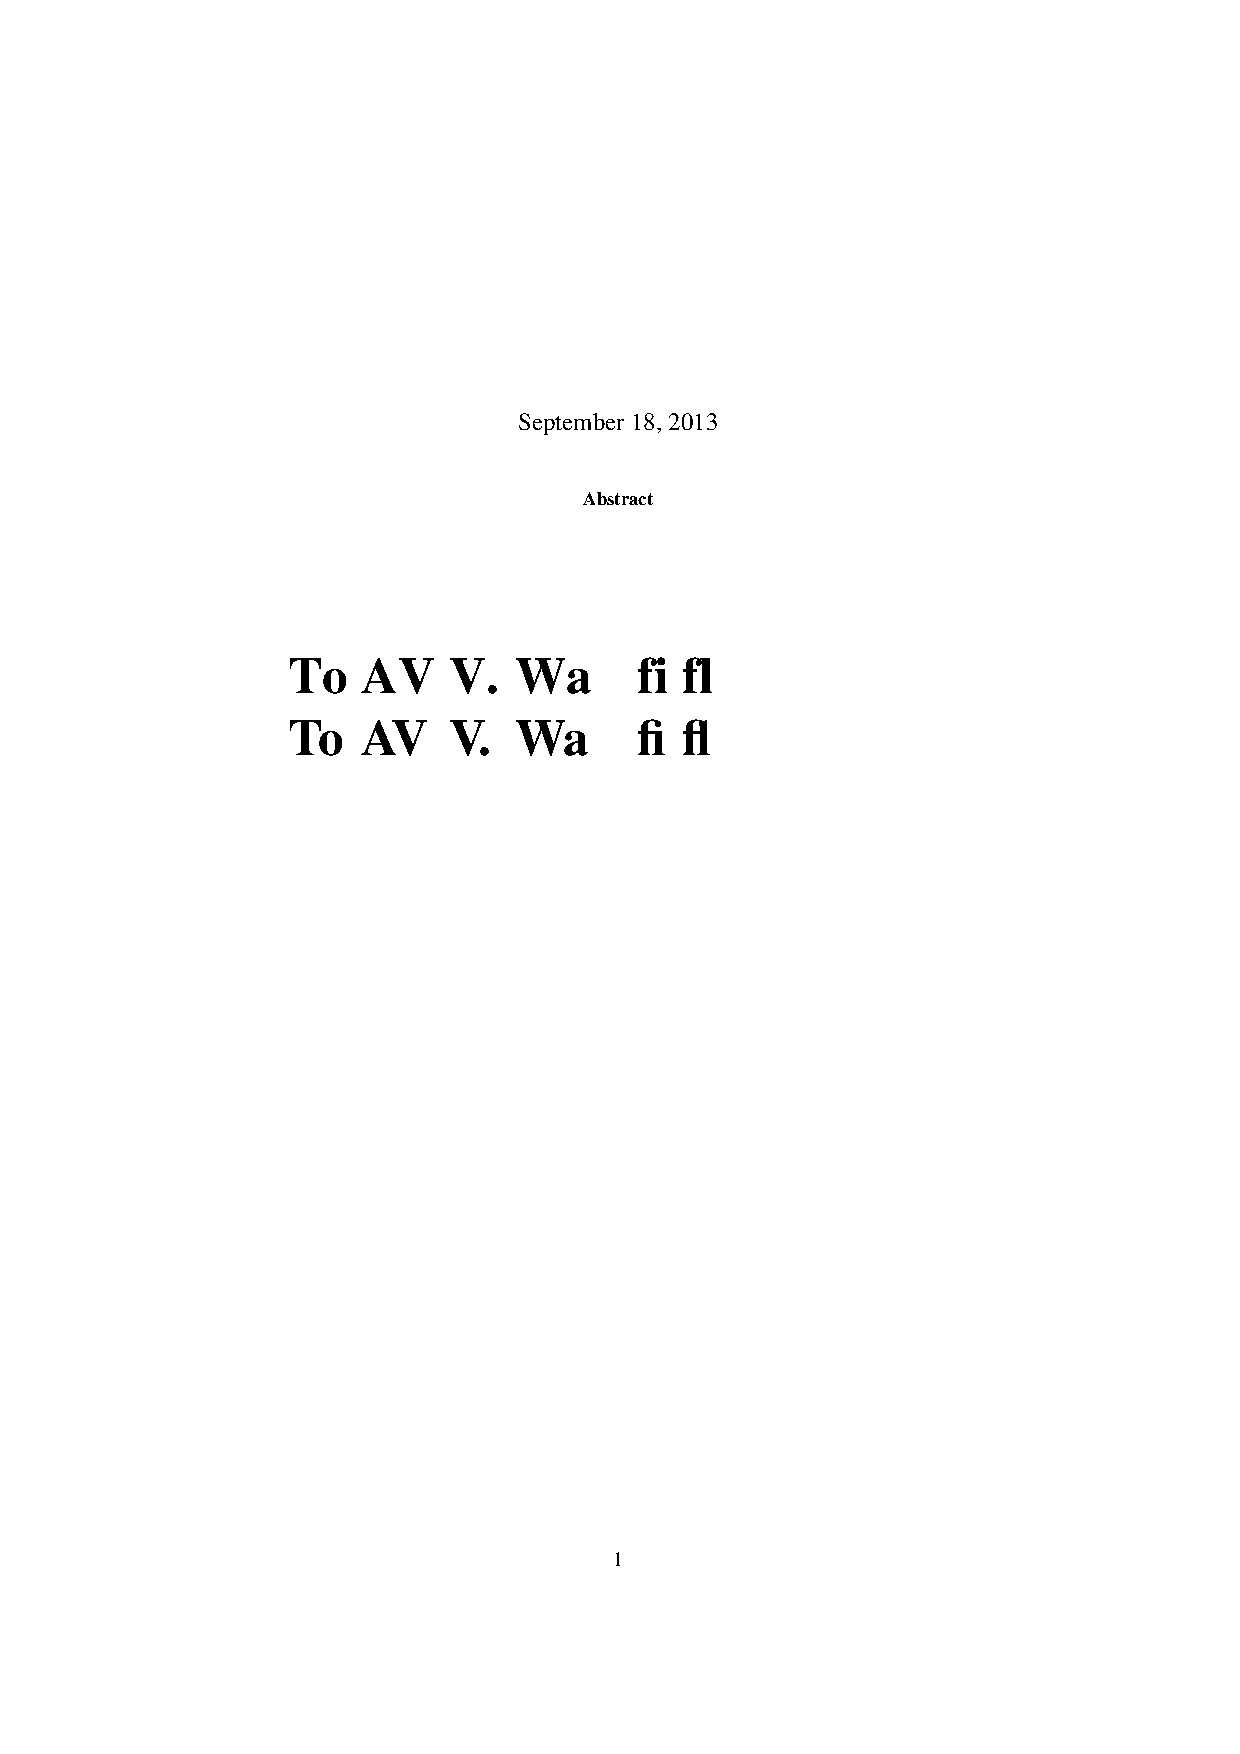
\includegraphics[trim=1.8in 6.54in 3.4in 4.25in, clip=true, width=\textwidth]{gfx/kerningetc}}
 \caption[Examples of microtypographical techniques]{Examples of various letter-pairs and their kerned (left) or ligature (right) equivalents, as typeset by pdf\LaTeX{}.}
 \label{fig:kern-lig}
\end{figure}

\subsection{Microtypographical Techniques}
Other techniques employed during hand-type\-set\-t\-ing and high-qua\-l\-ity electronic typesetting include the use of what is often termed \emph{micro\-typo\-graphy},~\cite{Hurst2009} for example, the use of kerning and ligatures. Kerning involves altering the spacing between certain glyph pairs in order to produce more consistent letter spacing, and ligatures are sin\-gle-glyph replacements for two or more single glyphs which may otherwise have clashing components. Some examples of these are shown in Figure~\ref{fig:kern-lig}.

Kerning requires a table of kern-pairs, specific to each font; values from this table must then be looked up for every pair of adjacent glyphs in the document. Ligatures may or may not need to be inserted: if the component characters of the ligature lie over a potential hyphenation point, it cannot be decided whether to replace them with the ligature until it is known whether the hyphenation point needs to be used. \TeX{} handles kerning and insertion of ligatures automatically, but there are still further typographical tweaks that its default typesetting algorithm does not use.

More advanced methods than simply stretching or shrinking the word spacing do exist, however. Robert Bringhurst, in \emph{The Elements of Typographic Style}~\cite{Bringhurst2008}, suggests that in addition to altering word spacing, subtle changes to inter-character spacing and individual glyph widths (in the range of $\pm$ 3\%) can produce more typographically and aesthetically pleasing results.

%pdf\LaTeX, used to typeset this thesis, \emph{does} make use of all the aforementioned techniques when performing text justification (unlike plain \TeX{} or \LaTeX{}).


\section{Summary}

We have so far seen that electronic representations of documents have layouts that are either fully fixed, or fully flowable. Currently there is no middle ground. Documents with fixed layouts may be of arbitrarily high typographic quality, since their layout is fully computed when they are created. Documents with flowable layouts are not provided with any guarantee that their content will be laid out with any semblance of typographic quality. In any case, to compute a high-quality layout in real-time is difficult, especially on a low-powered portable device such as an \ebook{} reader.

We have seen that screen technologies for \ebook{} readers have been evolving to become better and better, allowing documents to be displayed in a quality that rivals physical, printed pages. Document representation paradigms have not caught up. They are based on 1990s technology, and were never designed to be used in the way they are today. Fixed layout representations were designed for display on paper. Flowable layout representations were designed for display on such low-resolution screens (such as that in Figure~\ref{fig:calculator}) and underpowered devices that quality typography would have been nothing but a pipe dream.

It is time for a new document representation paradigm designed to match these new technologies\ed time for a \emph{malleable document format}.

It is proposed that by precomputing key parts of the typesetting process, a document may be afforded malleability, so that it may be gently coaxed to fit any page size, without compromising its typographic quality.

